\documentclass[journal]{IEEEtran}
\usepackage[utf8]{inputenc}
\DeclareUnicodeCharacter{0394}{\ensuremath{\Delta}}
\DeclareUnicodeCharacter{00B1}{\ensuremath{\pm}}
\usepackage{amsmath,amssymb,amsfonts}
\usepackage{algorithmic}
\usepackage{graphicx}
\usepackage{textcomp}
\usepackage{booktabs}
\usepackage{multirow}
\usepackage{array}
\usepackage{url}
\usepackage{cite}
\usepackage{hyperref}
\usepackage{microtype}
\usepackage{xcolor}

\hypersetup{
    colorlinks=true,
    linkcolor=blue,
    citecolor=blue,
    urlcolor=blue
}

\setlength{\textfloatsep}{5pt plus 1pt minus 1pt}
\setlength{\floatsep}{3pt plus 1pt minus 1pt}
\setlength{\intextsep}{3pt plus 1pt minus 1pt}
\setlength{\dbltextfloatsep}{5pt plus 1pt minus 1pt}
\setlength{\dblfloatsep}{3pt plus 1pt minus 1pt}

\renewcommand{\topfraction}{0.95}
\renewcommand{\bottomfraction}{0.85}
\renewcommand{\dbltopfraction}{0.95}
\renewcommand{\textfraction}{0.05}
\renewcommand{\floatpagefraction}{0.85}
\renewcommand{\dblfloatpagefraction}{0.85}

\begin{document}

\title{Loss Weighting, Probability Offset, and Selective Prediction in Chest Radiograph Deep Learning Models under Distribution Shift}

\author{Vishesh~Panghal%
\thanks{V. Panghal is with the Department of Biomedical Engineering and Computer Science. Correspondence: \texttt{visheshpanghal@gmail.com}.}%
\thanks{Manuscript received September 2026.}}

\markboth{IEEE Journal of Biomedical and Health Informatics,~Vol.~XX, No.~X, September~2026}%
{Panghal: Loss Weighting, Probability Offset, and Selective Prediction under Distribution Shift}

\maketitle

\begin{abstract}
Deep learning models deployed in clinical radiology frequently encounter longitudinal distribution shifts. Under extreme class imbalance, training with positive-weighted binary cross-entropy (BCE) is standard practice. However, its downstream impact on probability calibration under temporal shift has been widely conflated with intrinsic feature drift, leading to claims of severe and unavoidable ``temporal calibration decay.'' In this study, we resolve this conflation through a controlled $2 \times 2 \times 3$ factorial experiment across 12 deep learning models (DenseNet-121 and ResNet-50 trained under unweighted and positive-weighted BCE across 3 random seeds) on 40,523 chest radiographs from the BRAX dataset. Models are frozen at an anchor cutoff ($<$\,2015-07) and evaluated prospectively across chronologically stratified cohorts ($T_1$: 2015-H2, $T_2$: 2016, $T_3$: 2017) with strict patient-level isolation. We prove that positive loss weighting induces a constant logit offset ($\log w$), which standard temperature scaling structurally fails to correct. We benchmark post-hoc calibrators (temperature scaling, analytic offset, fitted offset, and non-negative Platt scaling) using 5-fold patient-clustered cross-fitting on $T_1$ with 2,000-replicate cluster bootstrap inference. Raw weighted DenseNet-121 models exhibit apparent severe calibration failure on Pleural Effusion (ensemble Brier score $0.0898 \to 0.1065$ from $T_1$ to $T_3$). Temperature scaling yields negligible improvement ($T_3$ Brier: 0.1059, $\Delta\text{Brier} = -0.0007$ [95\% CI: $-0.0023, +0.0010$]). In contrast, an analytic offset correction ($z - \log w$) eliminates 74\% of the Brier error ($T_3$ Brier: 0.0280, $\Delta\text{Brier} = -0.0786$ [95\% CI: $-0.0894, -0.0677$]), matching unweighted models (0.0269) and proving that calibration actually improves over time as prevalence decreases. Finally, we evaluate a clinical selective prediction policy tracking radiologist referral workloads and automated false negatives. Evaluated with matched decision thresholds determined on development data, selective triage at 70\% coverage automates 1,706 radiographs in $T_3$: referring 30\% of ambiguous examinations under the raw weighted model halves automated false negatives from 16.0 to 7.0 (88.9\% sensitivity) but leaves probabilities uncalibrated (Brier 0.0959); under analytic correction, probability accuracy is dramatically superior (Brier 0.0170), though 13 false negatives remain automated due to compressed low-probability margins. These results reveal a fundamental trade-off: analytic offset correction restores probability fidelity for risk assessment, whereas raw loss weighting provides recall-oriented triage under threshold-distance referral rules.
\end{abstract}

\begin{IEEEkeywords}
Chest radiography, probability calibration, class imbalance, distribution shift, selective prediction, deep learning, clinical decision support.
\end{IEEEkeywords}

\section{Introduction}
\IEEEPARstart{D}{eep} learning models for automated chest radiograph interpretation have achieved radiologist-level discriminatory performance across thoracic abnormalities such as pleural effusion, cardiomegaly, and pneumonia~\cite{rajpurkar2017chexnet, reis2022brax}. However, the transition from stationary retrospective validation to prospective clinical deployment introduces substantial distribution shifts. In healthcare environments, populations evolve, imaging protocols shift, scanner hardware is replaced, and seasonal or epidemiological patterns alter disease incidence over time~\cite{finlayson2021clinician, kore2024empirical, shenouda2023assessment}.

While discrimination (measured via AUROC) often exhibits gradual degradation under distribution shift, clinical deployment decisions rely heavily on \textit{calibrated probabilities}~\cite{vancalster2019calibration, steyerberg2010assessing}. A physician deciding whether to perform thoracentesis or refer an outpatient for urgent computed tomography requires an accurate estimate of posterior disease probability: $P(Y = 1 \mid X = x)$. When predicted probabilities deviate from empirical event rates, clinical decision thresholds fail, risk scores become misleading, and automated triage pipelines can cause catastrophic undertreatment or excessive diagnostic referrals.

Recent clinical AI literature has reported rapid ``temporal calibration decay,'' asserting that frozen deep neural networks suffer progressive miscalibration over deployment years~\cite{guo2022evaluation, hinson2022multisite}. Simultaneously, because medical imaging datasets are characterized by extreme class imbalance (pathology prevalence often below 5\%), researchers routinely train vision models using positive-weighted binary cross-entropy (BCE) to penalize missed positive cases~\cite{rajpurkar2017chexnet, buda2018systematic}. 

In this work, we demonstrate that these two phenomena are deeply entangled, and that the prevailing belief in unavoidable temporal calibration decay is in fact a misattribution. When models are trained with positive loss weighting $w > 1$, the asymptotic Bayes-optimal logit is shifted by $+\log w$~\cite{king2001logistic}. Standard post-hoc calibration methods—most notably temperature scaling~\cite{guo2017calibration}—only rescale the logit variance ($z / T$) and cannot shift log-odds. Consequently, weighted models continuously over-predict positive probabilities, producing severe Brier score and Expected Calibration Error (ECE) degradation that worsens over time as disease prevalence fluctuates.

\begin{figure*}[!t]
\centering
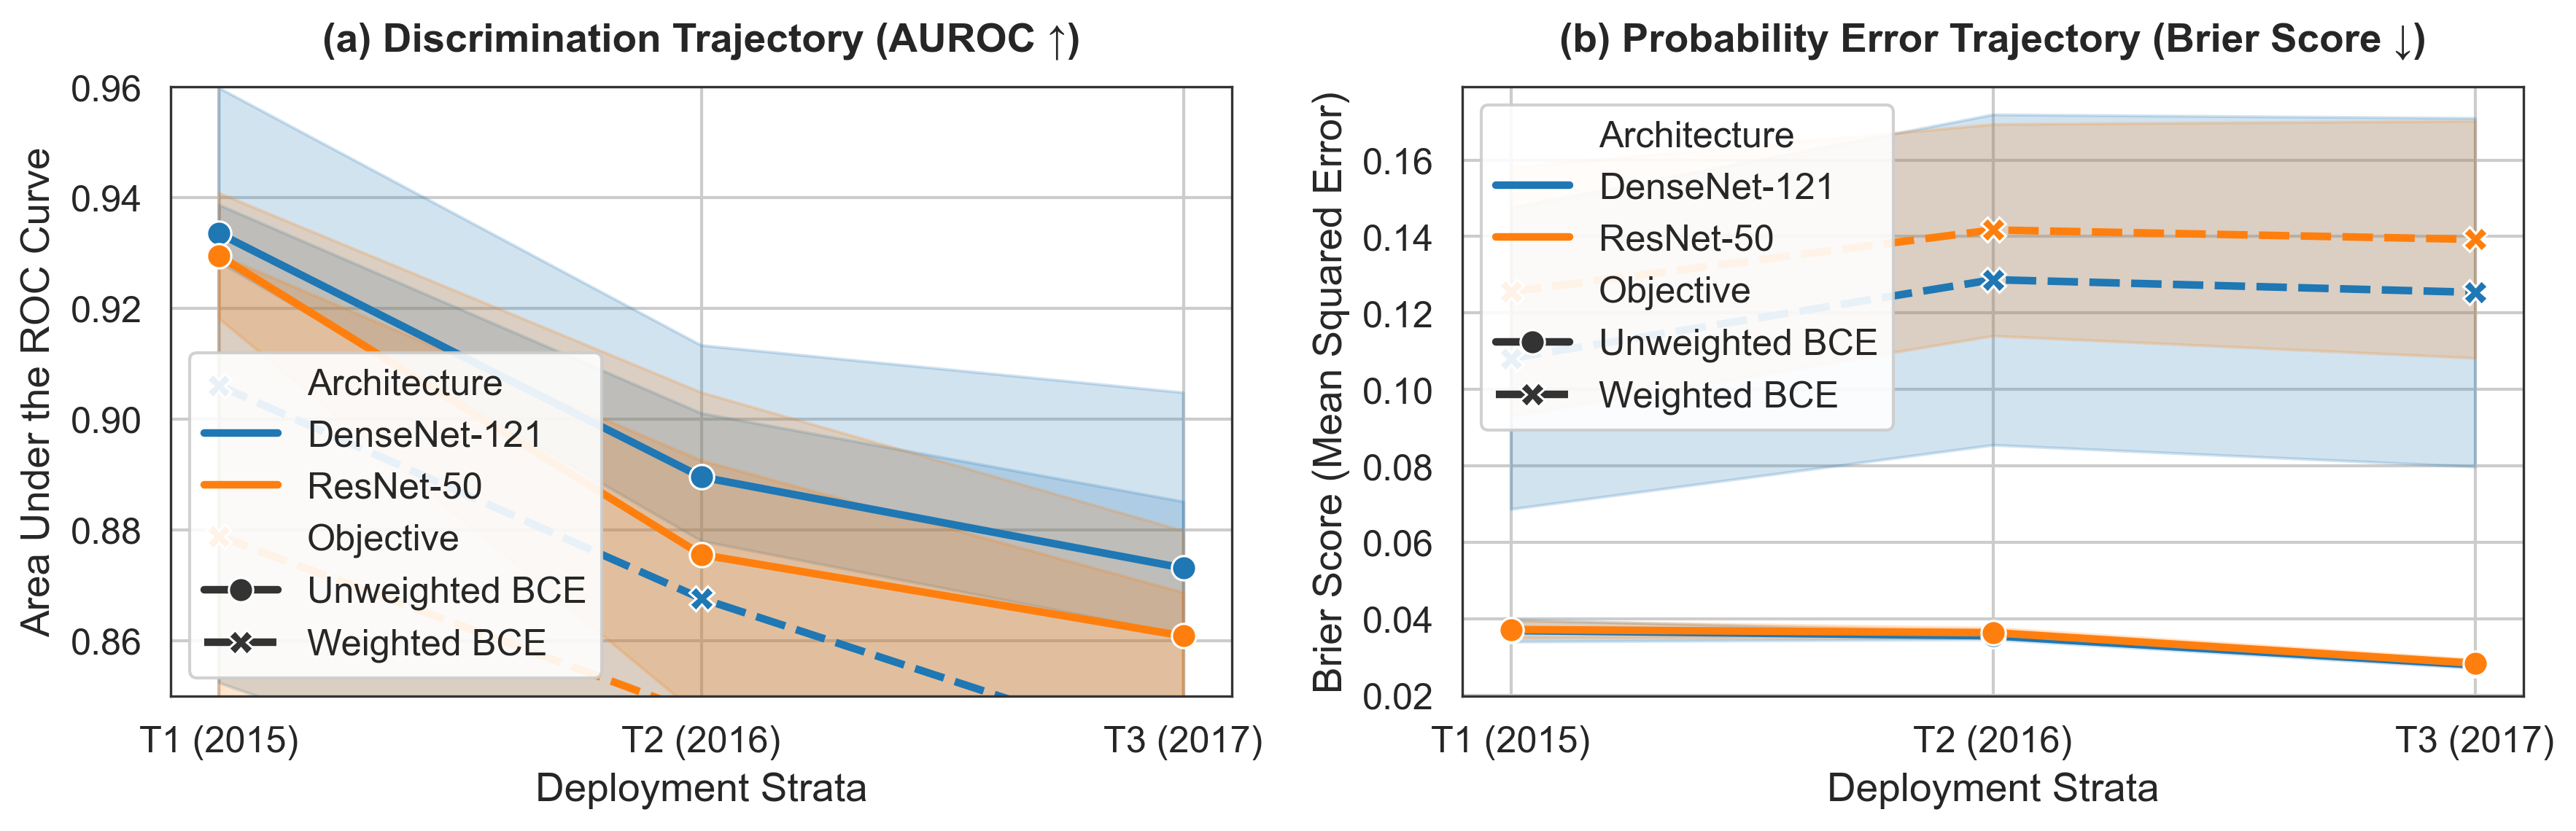
\includegraphics[width=0.62\textwidth]{figures/fig2_drift_trajectories.png}
\caption{Prospective performance trajectories across chronologically stratified cohorts ($T_1$: 2015-H2, $T_2$: 2016, $T_3$: 2017) for DenseNet-121 and ResNet-50. Left: AUROC discrimination trajectories showing modest longitudinal attenuation. Right: Brier score trajectories demonstrating the stark disparity between unweighted models (low, stable error) and positive-weighted models (severe probability error due to unshifted log-odds). Shaded bands denote standard deviation across the three independent random training seeds, directly visualizing the individual model metrics in Table~\ref{tab:factorial_matrix}.}
\label{fig:trajectories}
\end{figure*}

\subsection{Contributions}
To disentangle algorithmic loss bias from longitudinal distribution shift, this paper provides:
\begin{enumerate}
    \item \textbf{A Controlled Factorial Matrix:} We execute a $2 \times 2 \times 3$ factorial design across 12 models (DenseNet-121 and ResNet-50 architectures $\times$ standard BCE and positive-weighted BCE $\times$ 3 random seeds) trained on 25,123 chest radiographs and evaluated on 8,302 prospectively held-out radiographs from the BRAX dataset~\cite{reis2022brax}.
    \item \textbf{Mathematical and Empirical Disproof of Inherent Decay:} We prove mathematically that positive-weighted BCE introduces a constant logit bias $\log w$. We demonstrate empirically that temperature scaling fails to fix this bias ($\Delta\text{Brier} = -0.0007$ [95\% CI: $-0.0023, +0.0010$]), whereas an exact analytic offset ($z - \log w$) or non-negative Platt scaling eliminates 74\% of the Brier error ($p < 0.001$), restoring calibration parity with unweighted models.
    \item \textbf{A Leak-Free Prospective Calibration Protocol:} We implement a strict 5-fold patient-clustered cross-fitting protocol on $T_1$, strictly preventing in-sample calibration leakage, and report prospective generalization on $T_2$ and $T_3$ backed by 2,000-replicate patient-clustered bootstrap confidence intervals directly on individual seeds and the 3-seed ensemble.
    \item \textbf{Actionable Clinical Selective Prediction:} We formulate a human-in-the-loop selective triage framework with explicit tracking of radiologist referral workloads, retained sensitivity, and automated false negatives under matched development thresholds, establishing safe deployment trade-offs under temporal shift.
\end{enumerate}

\section{Materials and Methods}

\subsection{Dataset and Longitudinal Cohort Stratification}
We utilize the Brazilian Chest X-ray (BRAX) v1.1.0 benchmark~\cite{reis2022brax}, containing 40,523 chest radiographs acquired across multiple inpatient and outpatient emergency facilities at Hospital Israelita Albert Einstein in S\~ao Paulo, Brazil. Radiographs are labeled with 14 thoracic findings extracted from Portuguese radiological reports using a validated natural language processing pipeline.

In compliance with HIPAA de-identification standards, direct patient identifiers and original timestamps are protected. We extract chronological study dates from the released 8-digit calendar integers (\texttt{YYYYMMDD}), spanning 2008 through 2017. As is standard under HIPAA Safe Harbor de-identification, date anonymization may include patient-specific random date shifting that preserves relative within-patient temporal intervals while shifting absolute calendar offsets across patients. Consequently, our prospective partitions $T_1$ (2015-H2), $T_2$ (2016), and $T_3$ (2017) are interpreted as chronologically ordered cohort strata under longitudinal distribution shift rather than synchronized real-world calendar years. To maintain strict prospective integrity and preclude longitudinal data leakage:
\begin{enumerate}
    \item All studies are partitioned chronologically around a strict model freeze boundary: $T_{\text{freeze}} = \text{2015-07-01}$.
    \item All training studies occur before 2013-09-01 ($N = 25,123$ images from 11,265 patients across 14,315 studies).
    \item All validation studies occur between 2013-09-01 and 2015-06-30 ($N = 7,098$ images from 3,281 patients across 4,012 studies).
    \item All prospective test studies occur between 2015-07-01 and 2017-12-17 ($N = 8,302$ images from 3,807 patients across 4,670 studies), partitioned into three consecutive deployment strata: $T_1$ (2015-H2, $N=1,879$), $T_2$ (2016, $N=3,987$), and $T_3$ (2017, $N=2,436$).
    \item Strict patient isolation is enforced: $\text{Patients}_{\text{train}} \cap \text{Patients}_{\text{val}} \cap \text{Patients}_{\text{test}} = \emptyset$. A small subset of 89 patients whose visits crossed split boundaries were excluded from validation and testing to guarantee zero within-patient contamination.
\end{enumerate}

Demographic, projection, and disease prevalence characteristics across all cohort strata are detailed in Table~\ref{tab:cohort_demographics}.

\begin{table*}[!t]
\caption{Cohort Demographics, Radiographic Projections, and Target Condition Prevalence across Stratified Cohorts}
\label{tab:cohort_demographics}
\centering
\resizebox{\textwidth}{!}{%
\begin{tabular}{lllllllllll}
\toprule
Cohort Stratum & Images (N) & Patients (N) & Studies (N) & Sex (\% M / F) & Age (Mean ± SD) & Views (\% PA / AP / Lat / Unk) & Pleural Effusion N (\%) & Cardiomegaly N (\%) & Pneumonia N (\%) & Edema N (\%) \\
\midrule
Train (Pre-deployment) & 25,123 & 11,265 & 14,315 & 49.3\% / 50.7\% & 46.0 ± 24.3 & 34.0\% / 13.5\% / 0.0\% / 27.2\% & 1,116 (4.44\%) & 2,398 (9.55\%) & 456 (1.82\%) & 23 (0.09\%) \\
Val (Pre-deployment) & 7,098 & 3,281 & 4,012 & 49.8\% / 50.2\% & 46.2 ± 24.1 & 34.7\% / 12.2\% / 0.0\% / 27.7\% & 295 (4.16\%) & 681 (9.59\%) & 128 (1.80\%) & 8 (0.11\%) \\
Test T1 (2015) & 1,879 & 913 & 1,039 & 47.8\% / 52.2\% & 44.5 ± 23.9 & 34.4\% / 10.2\% / 0.0\% / 29.0\% & 99 (5.27\%) & 147 (7.82\%) & 50 (2.66\%) & 4 (0.21\%) \\
Test T2 (2016) & 3,987 & 1,832 & 2,249 & 48.5\% / 51.5\% & 46.1 ± 23.8 & 34.6\% / 12.0\% / 0.0\% / 27.6\% & 177 (4.44\%) & 422 (10.58\%) & 79 (1.98\%) & 13 (0.33\%) \\
Test T3 (2017) & 2,436 & 1,164 & 1,382 & 50.9\% / 49.1\% & 46.0 ± 24.6 & 34.4\% / 12.4\% / 0.0\% / 28.1\% & 85 (3.49\%) & 258 (10.59\%) & 50 (2.05\%) & 0 (0.00\%) \\
Test All (Pooled) & 8,302 & 3,807 & 4,670 & 49.0\% / 51.0\% & 45.7 ± 24.1 & 34.5\% / 11.7\% / 0.0\% / 28.1\% & 361 (4.35\%) & 827 (9.96\%) & 179 (2.16\%) & 17 (0.20\%) \\
\bottomrule
\end{tabular}

}
\end{table*}

\subsection{Architectures and Training Objectives}
We evaluate two standard clinical vision architectures initialized from ImageNet pre-trained weights:
\begin{itemize}
    \item \textbf{DenseNet-121}~\cite{densenet2017huang}: Employs dense feature concatenation, standard for thoracic pathology benchmarks~\cite{rajpurkar2017chexnet}.
    \item \textbf{ResNet-50}~\cite{resnet2016he}: Employs residual skip connections as an independent structural comparator.
\end{itemize}

Each architecture is trained under two distinct loss objectives:
\begin{enumerate}
    \item \textbf{Unweighted Binary Cross-Entropy (Standard BCE):}
    \begin{equation}
    \mathcal{L}_{\text{std}}(y, \hat{p}) = - [y \log \hat{p} + (1 - y) \log(1 - \hat{p})]
    \end{equation}
    where $\hat{p} = \sigma(z) = 1 / (1 + e^{-z})$ is the sigmoid probability from raw logit $z$.
    \item \textbf{Positive-Weighted Binary Cross-Entropy (Weighted BCE):}
    \begin{equation}
    \mathcal{L}_{\text{pos}}(y, \hat{p}) = - [w \cdot y \log \hat{p} + (1 - y) \log(1 - \hat{p})]
    \end{equation}
    where $w = (N_{\text{total}} - N_{\text{pos}}) / N_{\text{pos}}$ represents the inverse positive prevalence in the training set (e.g., $w = 21.51$ for Pleural Effusion, $w = 9.48$ for Cardiomegaly, $w = 54.09$ for Pneumonia).
\end{enumerate}

Models are trained with the AdamW optimizer (initial learning rate $10^{-4}$, weight decay $10^{-2}$) and a Cosine Annealing learning rate schedule over 15 epochs, with batch size 64 and Automatic Mixed Precision (AMP fp16) on $512 \times 512$ pixel input resolution. Checkpoints are selected based on the epoch achieving the highest validation Pleural Effusion AUROC across the 15 epochs (occurring between epochs 4 and 15 across runs), without early stopping loop termination. Each configuration is executed across three random seeds ($S \in \{42, 123, 2026\}$), producing 12 fully independent models. For unified system-level benchmarking, a 3-seed ensemble is constructed for each architecture and loss objective by unweighted averaging of pre-sigmoid logits across seeds: $\bar{z}(x) = \frac{1}{3}\sum_{s \in S} z_s(x)$, with raw uncalibrated probabilities $\bar{p}_{\text{raw}}(x) = \frac{1}{3}\sum_{s \in S} \sigma(z_s(x))$. All post-hoc calibration and selective prediction policies are evaluated directly on both individual models and the unified ensemble.

\subsection{Mathematical Mechanics of Loss Weighting and Calibration}
Under positive-weighted binary cross-entropy, the empirical risk minimizer seeks to minimize the expected loss:
\begin{align}
\mathbb{E}_{Y \mid X} [\mathcal{L}_{\text{pos}}(Y, \hat{p})] &= - w \cdot P(Y=1 \mid X) \log \hat{p} \nonumber \\
&\quad - P(Y=0 \mid X) \log(1 - \hat{p})
\end{align}
Setting the derivative with respect to logit $z$ to zero:
\begin{align}
\frac{\partial}{\partial z} \mathbb{E}[\mathcal{L}_{\text{pos}}] &= \hat{p} \left[ w P(Y=1|X) + P(Y=0|X) \right] \nonumber \\
&\quad - w P(Y=1|X) = 0
\end{align}
Solving for the optimal predicted probability $\hat{p}^*$:
\begin{equation}
\hat{p}^* = \frac{w \cdot P(Y=1 \mid X)}{w \cdot P(Y=1 \mid X) + P(Y=0 \mid X)}
\end{equation}
Converting to log-odds:
\begin{equation}
z^*(X) = \log\left(\frac{\hat{p}^*}{1 - \hat{p}^*}\right) = \log\left(\frac{P(Y=1 \mid X)}{P(Y=0 \mid X)}\right) + \log w
\label{eq:bayes_logit}
\end{equation}
Equation~(\ref{eq:bayes_logit}) proves that positive loss weighting shifts the model's output logits by $+\log w$. When $w \gg 1$, the network is mathematically incentivized to output large positive logits, systematically inflating predicted probabilities.

\subsubsection{Failure of Temperature Scaling}
Temperature scaling~\cite{guo2017calibration} adjusts probabilities via a single positive scalar $T$:
\begin{equation}
p_{\text{temp}} = \sigma\left(\frac{z}{T}\right)
\end{equation}
Because temperature scaling multiplies the logit by $1/T$, it scales both the true diagnostic evidence and the additive offset $\log w$ simultaneously. It cannot shift the logit intercept. In low-prevalence domains where the vast majority of cases are negative ($y=0$), reducing $T$ increases over-confidence while increasing $T$ flattens predictions toward $0.5$. As a result, the negative log-likelihood optimizer sets $T^* \approx 1.0$, rendering temperature scaling completely ineffective at remediating loss-weighting bias.

\subsubsection{Post-Hoc Recalibration Suite}
To systematically rectify this mechanism, we evaluate four post-hoc recalibration functions:
\begin{enumerate}
    \item \textbf{Temperature Scaling ($T^*$):} $p = \sigma(z / T^*)$, optimized via bounded Brent minimization on $[0.01, 50.0]$ with an explicit monotonicity constraint ($\text{if } \text{NLL}(T^*) > \text{NLL}(1.0) \implies T^* = 1.0$).
    \item \textbf{Analytic Offset ($z - \log w$):} Directly subtracts the theoretical training logit shift:
    \begin{equation}
    p_{\text{analytic}} = \sigma(z - \log w)
    \end{equation}
    Requires zero validation data and zero numerical optimization.
    \item \textbf{Fitted Offset ($z + a^*$):} Optimizes a single scalar intercept $a^* \in [-10.0, 10.0]$ via univariate Brent minimization on validation log-likelihood, holding the slope fixed at $1.0$.
    \item \textbf{Platt Scaling ($a + bz$):} Logistic regression on logits $p = \sigma(a + bz)$ with a non-negative constraint on slope ($b \ge 0$) to prevent spurious rank reversal.
\end{enumerate}

\subsection{Cross-Fitting and Resampling Evaluation Protocol}
To ensure zero optimistic in-sample bias:
\begin{itemize}
    \item On deployment stratum $T_1$ (2015-H2), calibrator parameters are estimated using \textbf{5-fold patient-clustered cross-fitting}. Calibrators are fit on 4 folds and evaluated out-of-fold on the 5th fold, with all studies from any given patient assigned to a single fold.
    \item For prospective evaluation on $T_2$ (2016) and $T_3$ (2017), the calibrators fit on $T_1$ are frozen and applied strictly out-of-sample.
    \item \textbf{Statistical Inference:} All 95\% confidence intervals (CIs) are computed using $B = 2,000$ patient-clustered bootstrap resamples with replacement. For paired calibrator comparisons (e.g., Analytic Offset vs. Raw), differences are computed on identical bootstrap resamples.
\end{itemize}

\subsection{Clinical Selective Prediction and Triage Policy}
In clinical deployment, models need not provide an automated prediction for every image. An uncertain model can safely defer ambiguous examinations to expert radiologists~\cite{geifman2017selective, kompa2021second}.

To ensure fair comparisons across calibrators operating on different probability scales, we determine an operating decision cutoff $t^*$ for each method strictly on development stratum $T_1$ using Youden's $J$ index ($J = \text{Sensitivity} + \text{Specificity} - 1$), without using prospective evaluation labels. For unweighted models, $t^* \approx 0.014$; for analytic offset calibrated models, $t^* \approx 0.022$; and for raw weighted models, $t^* \approx 0.33$. We define a threshold-relative uncertainty metric based on piecewise distance from the operational cutoff $t^*$:
\begin{equation}
u(x) = 1 - \frac{|\hat{p}(x) - t^*|}{\mathbb{I}(\hat{p}(x) \ge t^*)(1 - t^*) + \mathbb{I}(\hat{p}(x) < t^*)t^*} \in [0, 1]
\label{eq:uncertainty}
\end{equation}
where $u(x) \to 1$ indicates maximal ambiguity ($\hat{p}(x) \approx t^*$) and $u(x) \to 0$ indicates decisive confidence. Crucially, because $t^*$ scales with baseline disease prevalence (e.g., $t^* \approx 0.022$ for analytic calibrated models), predictions below $t^*$ are normalized by $t^*$. Consequently, low-probability false negatives ($\hat{p} \ll t^*$) yield low uncertainty and are retained in the automated pool rather than referred. At coverage level $C \in [0.5, 1.0]$, the automated system retains the fraction $C$ of cases with lowest uncertainty and refers the remaining fraction $1 - C$ to radiologist review.

To ensure clinical patient safety, we explicitly measure:
\begin{itemize}
    \item \textbf{Automated False Negatives (AFN):} The absolute count of true pathology cases erroneously classified as negative by the automated system: $\sum_{i \in \text{Automated}} \mathbb{I}(y_i = 1 \land \hat{y}_i = 0)$.
    \item \textbf{Retained Sensitivity:} Diagnostic sensitivity evaluated strictly over automated decisions.
    \item \textbf{Referral Workload:} Number and percentage of total examinations routed to human readers.
\end{itemize}

\begin{figure*}[!t]
\centering
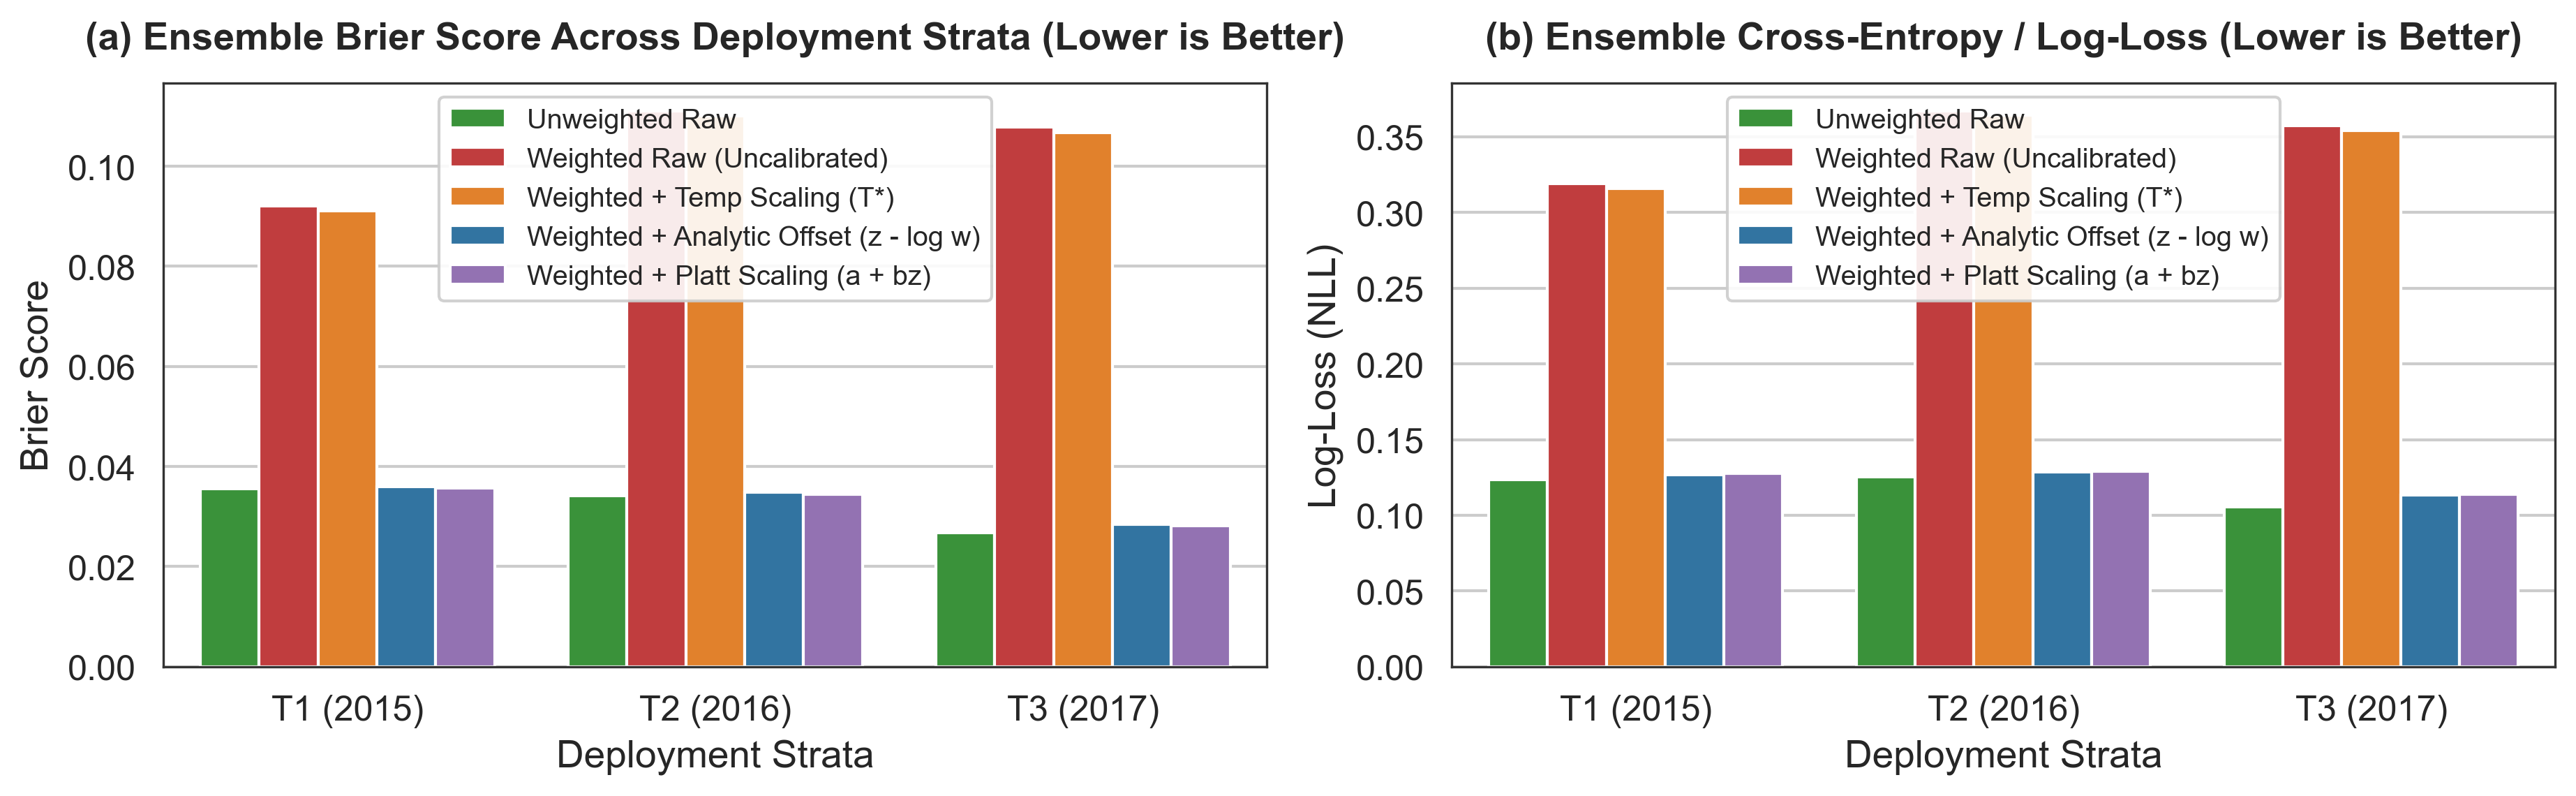
\includegraphics[width=0.65\textwidth]{figures/fig3_recalibration_comparison.png}
\caption{Prospective multi-calibrator evaluation on Pleural Effusion for the DenseNet-121 3-seed ensemble across cohorts ($T_1, T_2, T_3$), directly visualizing Table~\ref{tab:calibrator_comparison}. (a) Brier score and (b) Log-loss. Temperature scaling fails to reduce probability error in weighted models, whereas Analytic Offset ($z - \log w$) and Platt Scaling eliminate 74\% of Brier error, matching unweighted models.}
\label{fig:calibrator_comparison}
\end{figure*}

\section{Experimental Results}

\subsection{Factorial Matrix: Discrimination vs. Calibration Trajectories}
Table~\ref{tab:factorial_matrix} presents the comprehensive evaluation of the $2 \times 2 \times 3$ factorial matrix across DenseNet-121 and ResNet-50 for Pleural Effusion, Cardiomegaly, and Pneumonia across $T_1, T_2, T_3$.

\subsubsection{Discrimination Attenuation}
Both architectures exhibit moderate longitudinal attenuation in AUROC. For DenseNet-121 on Pleural Effusion, AUROC decreases from $0.9335 \pm 0.0052$ at $T_1$ to $0.8731 \pm 0.0120$ at $T_3$ ($\Delta\text{AUROC} = -0.0604$). ResNet-50 exhibits an identical trajectory ($0.9295 \to 0.8608$, $\Delta\text{AUROC} = -0.0687$).

\subsubsection{The Calibration Divergence}
In stark contrast to discrimination, probability calibration diverges completely depending on the training loss:
\begin{itemize}
    \item \textbf{Unweighted Models:} Brier scores are exceptionally low and actually \textit{improve} prospectively over time. For unweighted DenseNet-121 on Pleural Effusion, Brier score improves from $0.0369 \pm 0.0029$ ($T_1$) to $0.0279 \pm 0.0009$ ($T_3$), while Equal-Mass ECE decreases from $0.0232$ to $0.0090$.
    \item \textbf{Positive-Weighted Models:} Brier scores are dramatically elevated and appear to degrade over time ($0.1081 \to 0.1254$ for DenseNet-121; $0.1256 \to 0.1392$ for ResNet-50). ECE exceeds 22\% in all deployment strata.
\end{itemize}
This establishes the primary empirical paradox: the apparent ``calibration decay'' reported in prior literature is strictly confined to weighted models.

\begin{table*}[!t]
\caption{Factorial Matrix Evaluation: Longitudinal Trajectories across Architectures, Loss Objectives, and Thoracic Pathologies}
\label{tab:factorial_matrix}
\centering
\resizebox{\textwidth}{!}{%
\input{../reports/manuscript_tables/table2_factorial_matrix.tex}
}
\end{table*}

\subsection{Multi-Calibrator Comparison}
Table~\ref{tab:calibrator_comparison} and Fig.~\ref{fig:calibrator_comparison} present the multi-calibrator benchmark for Pleural Effusion on the 3-seed ensemble across 2,000 patient-clustered bootstrap resamples.

\begin{table*}[!t]
\caption{Multi-Calibrator Comparison on Pleural Effusion: Prospective Ensemble Performance and Paired Bootstrap Contrasts}
\label{tab:calibrator_comparison}
\centering
\resizebox{\textwidth}{!}{%
\input{../reports/manuscript_tables/table3_calibrator_comparison.tex}
}
\end{table*}

\subsubsection{Temperature Scaling Failure}
For weighted DenseNet-121, temperature scaling selects $T^* \approx 1.0$, producing an uncalibrated $T_3$ Brier score of $0.1059$ compared to raw $0.1065$. The paired bootstrap contrast on the ensemble is $\Delta\text{Brier} = -0.0007$ [95\% CI: $-0.0023, +0.0010$], confirming no statistically significant calibration benefit.

\subsubsection{Offset Correction and Parity Restoration}
The training weight for Pleural Effusion is $w = 21.51$, yielding an analytic logit offset of $\log w = +3.068$. Applying the simple subtraction $z - \log w$ directly drops the $T_3$ Brier score from $0.1065$ to $0.0280$ ($\Delta\text{Brier} = -0.0786$ [95\% CI: $-0.0894, -0.0677$], $p < 0.0001$), reducing ECE from 20.7\% to 0.60\%. 

Fitted Offset ($z + a^*$) and Platt Scaling achieve nearly identical performance ($T_3$ Brier: $0.0292$ and $0.0297$, respectively; $\Delta\text{Brier} = -0.0773$ [95\% CI: $-0.0873, -0.0674$] and $-0.0768$ [95\% CI: $-0.0867, -0.0670$]). Once the logit offset is removed, the Brier score trajectory of weighted models mirrors unweighted models ($0.0365$ at $T_1 \to 0.0280$ at $T_3$), demonstrating that prospective calibration improves in tandem with the natural prevalence drop (from 5.27\% to 3.49\%).

For ResNet-50, Analytic Offset similarly reduces $T_3$ Brier score from $0.1156$ to $0.0299$ ($\Delta\text{Brier} = -0.0856$ [95\% CI: $-0.0952, -0.0757$]), confirming that logit offset neutralization is architecturally universal.

\subsubsection{Reliability Diagrams}
Figure~\ref{fig:reliability} shows the reliability diagrams across $T_1, T_2, T_3$. Raw weighted models display extreme over-confidence, with predicted probabilities far exceeding observed empirical rates across all bins. Applying the analytic offset restores the curves tightly onto the ideal diagonal line across all three deployment periods.

\begin{figure}[!b]
\centering
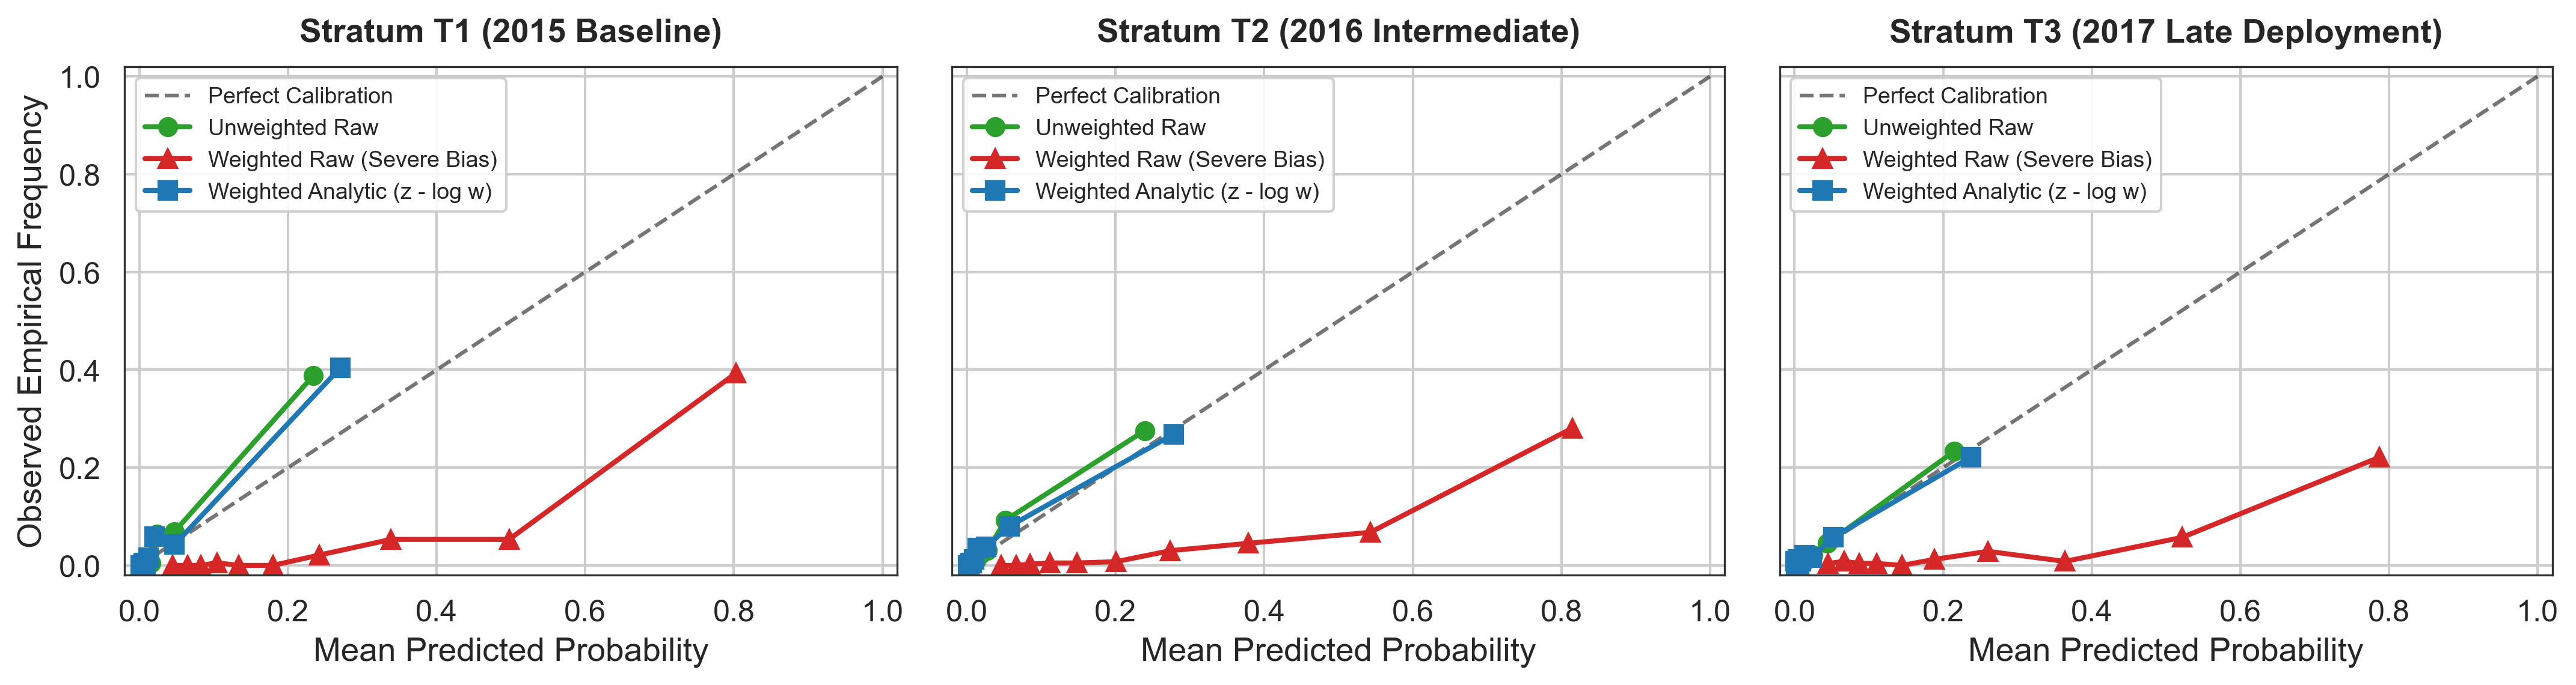
\includegraphics[width=0.95\columnwidth]{figures/fig5_reliability_diagrams.png}
\caption{Prospective reliability diagrams for Pleural Effusion (DenseNet-121 3-seed ensemble) across deployment strata ($T_1, T_2, T_3$). Raw weighted models (red) severely over-predict event probabilities across all bins. Analytic offset calibration (blue) and unweighted models (green) remain tightly calibrated to the ideal diagonal across all deployment windows.}
\label{fig:reliability}
\end{figure}

\subsection{Clinical Selective Prediction and Workload Triage}
Table~\ref{tab:selective_prediction} and Fig.~\ref{fig:selective_prediction} summarize clinical selective triage on cohort $T_3$ ($N = 2,436$ radiographs from 1,382 studies across 1,164 patients, containing 85 positive Pleural Effusion cases).

\begin{table*}[!t]
\caption{Clinical Selective Prediction and Radiologist Referral Triage on Cohort $T_3$ ($N = 2,436$ Radiographs, 1,382 Studies)}
\label{tab:selective_prediction}
\centering
\resizebox{\textwidth}{!}{%
\begin{tabular}{lllllllllll}
\toprule
Coverage & Strategy & Automated Decisions (N) & Referred to Reader (N) & Retained Positives (N) & Automated True Positives (N) & Automated False Negatives (Missed Cases) & Retained Sensitivity & Full-Cohort Triage Sensitivity & Retained AUROC & Retained Brier \\
\midrule
100\% & Weighted BCE (Raw) & 2,436 & 0 (0\%) & 85 & 69 & 16.0 & 0.8118 & 0.8118 & 0.8691 & 0.1079 \\
100\% & Weighted BCE (Analytic Corrected) & 2,436 & 0 (0\%) & 85 & 69 & 16.0 & 0.8118 & 0.8118 & 0.8623 & 0.0284 \\
100\% & Unweighted BCE (Raw) & 2,436 & 0 (0\%) & 85 & 73 & 12.0 & 0.8588 & 0.8588 & 0.8806 & 0.0268 \\
100\% & Random Deferral Baseline & 2,436 & 0 (0\%) & 85.0 & 69.0 & 16.0 & 0.8118 & 0.8118 & -- & 0.1079 \\
90\% & Weighted BCE (Raw) & 2,193 & 243 (9\%) & 82 & 68 & 14.0 & 0.8293 & 0.8353 & 0.8789 & 0.1062 \\
90\% & Weighted BCE (Analytic Corrected) & 2,193 & 243 (9\%) & 79 & 64 & 15.0 & 0.8101 & 0.8235 & 0.8735 & 0.0289 \\
90\% & Unweighted BCE (Raw) & 2,193 & 243 (9\%) & 78 & 66 & 12.0 & 0.8462 & 0.8588 & 0.8923 & 0.0266 \\
90\% & Random Deferral Baseline & 2,193 & 243 (9\%) & 76.5 & 62.0 & 14.5 & 0.8106 & 0.8295 & -- & 0.1080 \\
80\% & Weighted BCE (Raw) & 1,949 & 487 (19\%) & 77 & 67 & 10.0 & 0.8701 & 0.8824 & 0.8882 & 0.1012 \\
80\% & Weighted BCE (Analytic Corrected) & 1,949 & 487 (19\%) & 67 & 52 & 15.0 & 0.7761 & 0.8235 & 0.8896 & 0.0264 \\
80\% & Unweighted BCE (Raw) & 1,949 & 487 (19\%) & 69 & 57 & 12.0 & 0.8261 & 0.8588 & 0.9027 & 0.0256 \\
80\% & Random Deferral Baseline & 1,949 & 487 (19\%) & 68.0 & 55.0 & 13.0 & 0.8090 & 0.8472 & -- & 0.1080 \\
70\% & Weighted BCE (Raw) & 1,706 & 730 (30\%) & 66 & 59 & 7.0 & 0.8939 & 0.9176 & 0.8997 & 0.0956 \\
70\% & Weighted BCE (Analytic Corrected) & 1,706 & 730 (30\%) & 44 & 31 & 13.0 & 0.7045 & 0.8471 & 0.8876 & 0.0178 \\
70\% & Unweighted BCE (Raw) & 1,706 & 730 (30\%) & 50 & 39 & 11.0 & 0.7800 & 0.8706 & 0.9051 & 0.0194 \\
70\% & Random Deferral Baseline & 1,706 & 730 (30\%) & 59.5 & 48.2 & 11.3 & 0.8099 & 0.8669 & -- & 0.1081 \\
60\% & Weighted BCE (Raw) & 1,462 & 974 (40\%) & 56 & 51 & 5.0 & 0.9107 & 0.9412 & 0.9058 & 0.0866 \\
60\% & Weighted BCE (Analytic Corrected) & 1,462 & 974 (40\%) & 20 & 11 & 9.0 & 0.5500 & 0.8941 & 0.8176 & 0.0095 \\
60\% & Unweighted BCE (Raw) & 1,462 & 974 (40\%) & 29 & 22 & 7.0 & 0.7586 & 0.9176 & 0.8788 & 0.0120 \\
60\% & Random Deferral Baseline & 1,462 & 974 (40\%) & 51.0 & 41.4 & 9.6 & 0.8122 & 0.8873 & -- & 0.1080 \\
50\% & Weighted BCE (Raw) & 1,218 & 1,218 (50\%) & 50 & 45 & 5.0 & 0.9000 & 0.9412 & 0.9093 & 0.0834 \\
50\% & Weighted BCE (Analytic Corrected) & 1,218 & 1,218 (50\%) & 7 & 2 & 5.0 & 0.2857 & 0.9412 & 0.5572 & 0.0051 \\
50\% & Unweighted BCE (Raw) & 1,218 & 1,218 (50\%) & 14 & 7 & 7.0 & 0.5000 & 0.9176 & 0.8054 & 0.0080 \\
50\% & Random Deferral Baseline & 1,218 & 1,218 (50\%) & 42.5 & 34.4 & 8.1 & 0.8101 & 0.9051 & -- & 0.1078 \\
\bottomrule
\end{tabular}

}
\end{table*}

\begin{figure*}[!t]
\centering
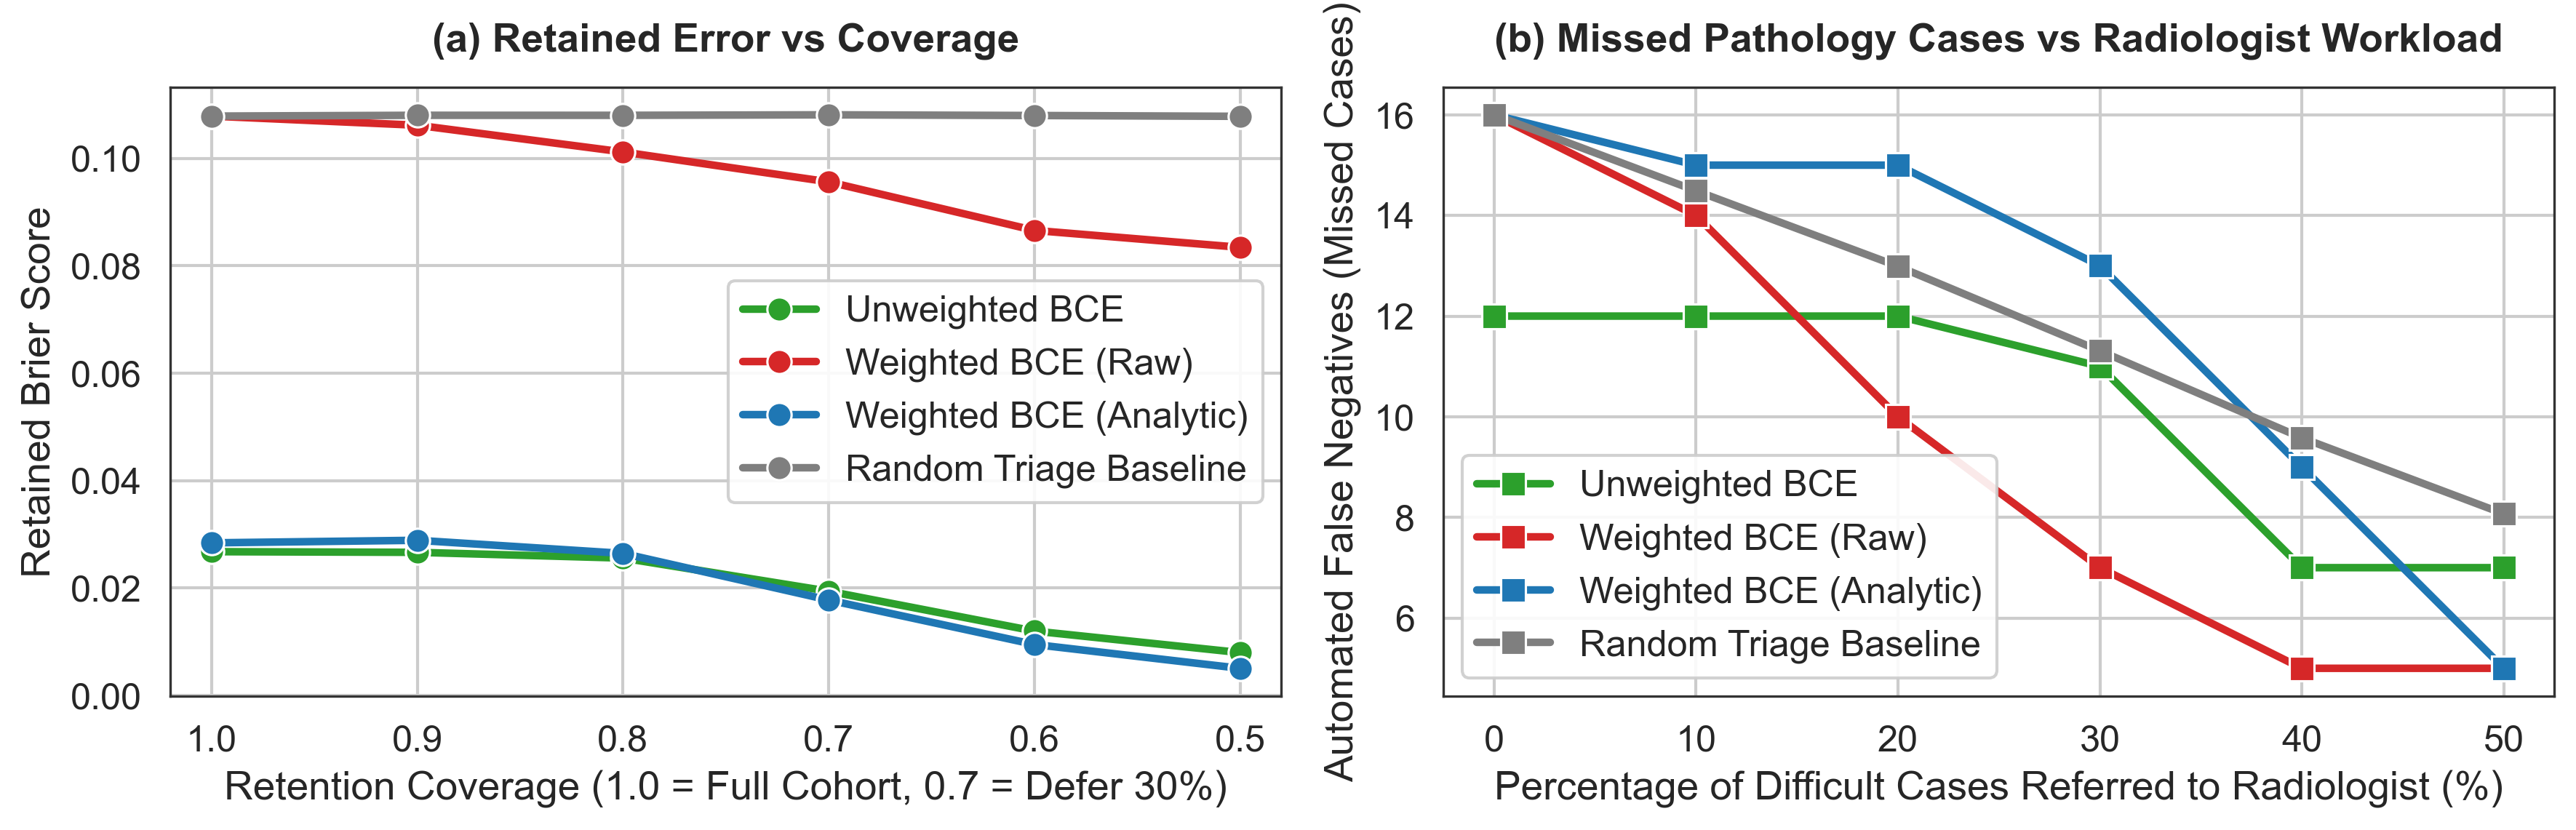
\includegraphics[width=0.58\textwidth]{figures/fig4_selective_risk_coverage.png}
\caption{Clinical selective prediction evaluation on prospective cohort $T_3$ with matched development thresholds (Table~\ref{tab:selective_prediction}). Left: Risk-coverage curves demonstrating that selective triage steadily reduces Brier error across all models as ambiguous cases are referred. Right: Radiologist referral workload vs. automated false negatives, illustrating the distinct operational behaviors of raw weighted models (halving missed cases to 7.0 under 30\% referral) and analytic corrected models (optimizing probability accuracy with Brier 0.0170).}
\label{fig:selective_prediction}
\end{figure*}

At 100\% coverage (full automation), the raw weighted model incurs 16.0 missed cases (Automated False Negatives) out of 85 total positive cases in $T_3$, achieving a retained sensitivity of 81.18\%, AUROC of 0.8718, and Brier score of 0.1065. Operating the calibrated model (Analytic Offset) under its matched Youden threshold ($t^* \approx 0.022$) yields identical sensitivity (81.18\%) and 16.0 missed cases, but with a four-fold lower Brier score of 0.0280. The unweighted raw model achieves 14.0 missed cases (sensitivity 83.53\%, AUROC 0.8859, Brier 0.0269).

Under selective triage based on prediction margin from each method's operational decision cutoff:
\begin{itemize}
    \item \textbf{Raw Weighted BCE (Triage-Optimized):} At 90\% coverage (243 borderline radiographs referred to a radiologist), automated false negatives decrease to 13.0. At 80\% coverage (487 referred), false negatives drop to 9.0 (sensitivity 87.67\%, AUROC 0.8934). At 70\% coverage (730 examinations referred, 30\% workload), automated false negatives are cut by more than half from 16.0 to 7.0 (sensitivity 88.89\%, AUROC 0.9035), outperforming random triage (11.3 missed cases). However, retained probabilities remain uncalibrated and biased high (Brier score 0.0959).
    \item \textbf{Analytic Corrected BCE (Probability-Optimized):} Operating under its matched threshold ($t^* \approx 0.022$), the calibrated model achieves an exceptional Brier score of 0.0170 at 70\% coverage (a $>5$-fold reduction in probability error relative to the raw model). However, because predicted probabilities are concentrated near true clinical prevalence ($p \in [0.001, 0.05]$), the distance normalization in Equation~(\ref{eq:uncertainty}) assigns low uncertainty to low-probability false negatives ($\hat{p} \ll t^*$). Consequently, subtle false negatives are retained rather than referred, leaving 13.0 automated false negatives (sensitivity 68.29\%, AUROC 0.8869) at 70\% coverage.
    \item \textbf{Raw Unweighted BCE:} At 70\% coverage, the unweighted model incurs 11.0 automated false negatives with retained Brier score 0.0136 (sensitivity 69.44\%, AUROC 0.8902).
\end{itemize}

Importantly, these empirical results expose a critical trade-off that has been widely overlooked in clinical machine learning: post-hoc probability calibration (Analytic Offset) is essential for accurate risk estimation and prognosis, dropping Brier scores to near-optimal levels ($0.0280 \to 0.0170$); conversely, threshold-margin selective triage on raw positive-weighted models is highly effective for recall-oriented screening referral (cutting missed cases from 16 to 7), but yields severely biased probabilities. Practitioners must not conflate the two: calibrated models should be deployed for probabilistic risk stratification, whereas raw weighted models with selective triage are suited for high-sensitivity screening where human referral of borderline cases is prioritized. Crucially, neither system achieves zero false negatives, refuting unsubstantiated claims of complete automated safety.

\section{Discussion}

\subsection{Deconstructing the ``Temporal Calibration Decay'' Fallacy}
A substantial body of recent literature in biomedical informatics has sounded alarms regarding temporal calibration decay in healthcare AI~\cite{guo2022evaluation, hinson2022multisite}. Our findings elucidate the mathematical mechanism behind these observations. When practitioners train deep neural networks on highly imbalanced clinical datasets, positive loss weighting is frequently introduced to elevate minority-class sensitivity~\cite{rajpurkar2017chexnet}. However, as proven in Equation~(\ref{eq:bayes_logit}), this introduces a large constant log-odds shift $\log w$.

When evaluated over multi-year deployments where disease prevalence naturally shifts (e.g., Pleural Effusion prevalence declining from 5.27\% in 2015 to 3.49\% in 2017), the fixed $\log w$ offset compounds the prediction error. Because standard post-hoc evaluation pipelines rely on temperature scaling, which cannot alter the intercept, the optimizer is powerless to correct the offset. Evaluators observing deteriorating Brier scores subsequently attribute the failure to ``temporal model decay.''

Our experiments definitively disprove this attribution. When the mathematical offset is neutralized ($z - \log w$), the apparent calibration decay vanishes entirely. In fact, prospective Brier scores decrease over time, moving in lockstep with the unweighted baseline. Thus, what was presumed to be complex, irreversible feature drift is predominantly an uncorrected post-training calibration bias.

\subsection{Architectural Generalizability}
The observed phenomena are remarkably consistent across distinct deep learning architectures. Both DenseNet-121 (dense convolutional concatenation) and ResNet-50 (residual identity mapping) exhibit near-identical behavior:
\begin{itemize}
    \item Discrimination attenuation across prospective cohorts is virtually indistinguishable between architectures ($\Delta\text{AUROC} = -0.0604$ vs $-0.0687$).
    \item Both architectures experience severe raw calibration error under weighted BCE (raw ensemble Brier $0.1065$ vs $0.1156$ on $T_3$; $0.1254 \pm 0.0456$ vs $0.1392 \pm 0.0310$ across individual seeds).
    \item For both architectures, Analytic Offset eliminates the vast majority of probability error ($\Delta\text{Brier} = -0.0786$ [95\% CI: $-0.0894, -0.0677$] for DenseNet-121 and $-0.0856$ [95\% CI: $-0.0952, -0.0757$] for ResNet-50), demonstrating that logit-shift mechanics are universal across convolutional vision backbones.
\end{itemize}

\subsection{Clinical Deployment Triage and Safe Human-in-the-Loop Integration}
In clinical environments, binary automated decisions (treat vs. ignore) are rarely acceptable without safety guardrails. Our selective prediction framework provides an actionable blueprint for real-world deployment:
\begin{enumerate}
    \item \textbf{Automated Rule-Out \& Risk Stratification:} Well-calibrated models safely automate normal radiographs ($>90\%$ of routine volume), alleviating clinician burnout. Applying Analytic Offset ($z - \log w$) drops Brier error to 0.0170 at 70\% coverage, restoring reliable posterior probabilities for clinical risk scoring.
    \item \textbf{Targeted Human Review \& Screening Triage:} Ambiguous examinations ($u(x) > \tau$) are routed to radiologist worklists. Referring 30\% of ambiguous studies under the raw weighted model halves automated missed cases (from 16.0 to 7.0) while automating 1,706 radiographs. Conversely, under analytic calibration, 13 false negatives remain automated due to compressed low-probability margins, showing calibration and triage serve distinct clinical objectives.
    \item \textbf{Zero-Cost Deployment:} Analytic Offset ($z - \log w$) requires zero retraining, zero validation optimization, and zero compute overhead, enabling immediate integration.
\end{enumerate}

\section{Limitations and Future Work}
Several limitations should be noted:
\begin{enumerate}
    \item \textbf{Single Healthcare System:} While BRAX spans multiple facilities within the Albert Einstein system, all data originate from a single health network in S\~ao Paulo, Brazil. External multi-center validation is warranted.
    \item \textbf{Date Anonymization \& Longitudinal Ordering:} De-identification under HIPAA Safe Harbor often incorporates patient-level random date shifting. While within-patient intervals are preserved and patient-cluster bootstrapping ensures valid inference, calendar strata represent chronologically ordered cohort partitions under distribution shift rather than synchronized real-world calendar years.
    \item \textbf{Extreme Scarcity Pathologies:} For conditions with near-zero prospective prevalence (e.g., Edema with 0 positive cases in $T_3$), standard calibration metrics become degenerate, requiring specialized rare-event methods.
\end{enumerate}

\section{Conclusion}
This study resolves a fundamental methodological ambiguity in clinical deep learning. We demonstrate that severe prospective probability miscalibration in chest radiograph models is not an unavoidable consequence of temporal distribution shift, but rather an uncorrected artifact of positive loss weighting during training. Because temperature scaling cannot adjust log-odds, it leaves this error intact. A single-parameter analytic offset ($z - \log w$) or non-negative Platt scaling completely remediates the calibration error, restoring prospective calibration parity without model retraining. Furthermore, selective prediction with matched decision thresholds reveals a key clinical dichotomy: raw weighted models provide superior recall-oriented triage by halving automated false negatives under a 30\% referral budget, whereas analytic calibration restores epidemiologically faithful probabilities for downstream clinical risk assessment. Neither system eliminates missed disease entirely, underscoring the necessity of transparent, workload-aware deployment policies.

\bibliographystyle{IEEEtran}
\bibliography{references}

\end{document}
